\documentclass{article}

% include graph
\usepackage{graphicx}
% if then else
\usepackage{ifthen}
% for sub itermize
\usepackage{outlines}
% using color package
\usepackage[usenames,dvipsnames]{color}
% 用于产生一种数学用的花体字  
\usepackage{mathrsfs}
% 数学符号  
\usepackage{amsmath,amssymb}
% 专门处理数学粗体的bm宏包
\usepackage{bm}
% 高质量数学字体/黑体  
\usepackage[cmintegrals]{newtxmath}
% Expectation by \E
% just use "\mathbb{E}"
% \DeclareMathOperator{\E}{\mathbb{E}}
% 英文花体, e.g., $\mathcal{D}$
% use table
\usepackage{tabularx}
\usepackage{booktabs}
% use tab
\usepackage{tabto}
% 可以换行的 \underline{}
% \usepackage{ulem}
%----------------------------- THE ARTICLE -------------------------------

\begin{document}

\begin{titlepage}
    \includegraphics[height=3.4cm]{../others/sedes.pdf}
    \\ \\
    \textbf{Fundamentals of Artificial Intelligence [H02C1a]}
    \\ \\ 
    \textbf{Xinhai Zou (r0727971)}
\end{titlepage}

\pagenumbering{roman} 
\tableofcontents
\clearpage
\pagenumbering{arabic}
\setcounter{page}{1}

\section{Intro to AI}
\subsection{Overview}
AI starts from \textbf{1955} in Bell Telephone Laboratories.
What is AI today?
\begin{outline}
    \1 Planning \& Scheduling
    \1 Declarative Programming
    \1 Robotics
    \1 Computer vision
    \1 Machine learning
    \1 language processing
    \1 Human computer interaction
    \1 theorem proving
\end {outline}
Sometime, we must make a decision when faced with insufficient information.
Being rational means maximizing your expected utility.
\subsection{Summary}
\begin{enumerate}
    \item One summer was not enough to shape AI -> but many significant advances have been made since!
    \item Movie AI, News AI and Research AI differ
    \item Modern AI systems combine 'reasoning' with 'learning' -> this course: 'resoning' focus
    \item Much to say about ethics and fairness of AI systems
\end{enumerate}
\pagebreak
\section{Rational agent}
\subsection{Overview}
\begin{outline}
    \1 Rational agent
        \2 Agent: an entity that perceives (from env.) and acts (to env.)
        \2 Rational: maximizing expected utility
        \2 Rational agent: selects actions that maximize its (expected) utility, i.e., they do the right thing.
    \1 Different environments
        \2 Accessible vs. inaccessible (fully observable vs. partially observable)
            \3 environment is fully observed by agent?
        \2 dterministic vs. stochasitic 
            \3 is the next state of the envioronment completely determined by the current state?
        \2 episodic vs. sequential
            \3 can the quality of an action be evaluated within \textbf{an episode} (perception + action)?
        \2 static vs. dynamic
            \3 can the environment change while the agent is deliberating?
            \3 dynamic - not turn-based game, static - mostly turn-based game
        \2 discrete vs. continuous
            \3 is the value discrete (nominal) or continuous (numerical)
        \2 single vs. multi-agent
            \3 which entities have to regarded as agents? (competitive or cooperative scenarios?)
\end{outline}

Example 
\begin{table}[htbp]\footnotesize
    \centering
    \caption{Examples using different environments}
    \begin{tabularx}{15cm}{X|XXXXXX}
    \toprule
    \textbf{Env.}&\textbf{Observable}&\textbf{Agents}&\textbf{Deterministic}&\textbf{Episodic}&\textbf{Static}&\textbf{Discrete} \\
    \hline
    \textbf{Crossword puzzle}&Fully&Single&Deterministic&\textcolor{red}{sequential}&\textcolor{red}{Static}&Discrete \\
    \hline
    \textbf{Chess with a clock}&&&&&& \\
    \hline
    \textbf{Poker}&&&&&& \\
    \hline
    \textbf{Backgammon}&&&&&& \\
    \hline
    \textbf{Taxi driving}&&&&&& \\
    \hline
    \textbf{Medical diagnosis}&&&&&& \\
    \hline
    \textbf{Image analysis}&&&&&& \\
    \hline
    \textbf{Part-picking robot}&&&&&& \\
    \hline
    \textbf{Refinery controller}&&&&&& \\
    \hline
    \textbf{English tutor}&&&&&& \\
    \hline
    \textbf{Pac-Mac}&Observable&Multi&\textcolor{red}{Stochasitic}&Sequential&\textcolor{red}{Dynamic}&Discrete \\
    \bottomrule
    \end{tabularx}
    \label{tab:diff_classification_association_rules}
\end{table}

\begin{outline}
    \1 Reflex agents
        \2 choose (respond) action only based on current state
        \2 do not consider the future consequences of their actions
    \1 Planning/ Goal based agent
        \2 choose action based on consequences of actions (future)
        \2 consider how the world will be
\end{outline}

\subsection{Summary}
\begin{enumerate}
    \item an agent is something that perceives and acts, being rational is to obtain maximal expected value. An rational agent will take the action that maximizes its expected performance given the percept sequence and its knowledge of the environment.
    \item an agent program maps from a percept to an action
    \begin{enumerate}
        \item reflex agents respond based on current state
        \item goal-based agents respond based on current and future state
        \item learning agents improve their behaviour over time
    \end{enumerate}
    \item some environments are more demanding than others
\end{enumerate}

\pagebreak
\section{State space}
\subsection{Overview}
How to represent a problem in machine? For a basic search problem, there are five ingredients.
\begin{enumerate}
    \item States: represent the states in a clear way
    \item Actions: define the actions you can execute and change the world state, normally $\delta: X \rightarrow Y$
    \item Initial state: what is the initial state, the \textbf{starting} point
    \item Goal formulation: define which states you want to end
    \item Specification of the search cost: the execution costs
\end{enumerate} 

\noindent
Take Pac-man - path-finding as an example, which is shown below:
\begin{outline}
    \1 States: $(x,y)$, where x is x-axis and y is y-axis
    \1 Initial state: starting point $(x_{0},y_{0})$
    \1 Actions: different actions
        \2 east: $f_{east}: (x,y) \rightarrow (x+1,y)$
        \2 west: $f_{west}: (x,y) \rightarrow (x-1,y)$
        \2 north: $f_{north}: (x,y) \rightarrow (x,y+1)$
        \2 south: $f_{south}: (x,y) \rightarrow (x,y-1)$
    \1 Goal test: goal point/state $(x^{*},y^{*})$
    \1 Path cost: each step cost 1 step unit, only have <specific number> state unit
\end{outline}

\noindent
Sometimes, we need a check-loop detection. We have two different structure for state-space representation: graph and search tree.
\begin{outline}
    \1 graph
        \2 For graph, during searching, we often keep track of the already visited nodes to avoid loops and redundancies.
    \1 search tree
        \2 nodes show states, each node in the search tree is an entire PATH in the state space graph.
\end{outline}

\noindent
Some key issues:
\begin{outline}
    \1 definition of state space and transition model
    \1 choose implicit graph or implicit tree
    \1 search forward or backward
    \1 use optimal solution or any solution
    \1 decompose difficult problem to simpler problem (problem reduction/ decomposability)
\end{outline}

\noindent
For forward and backward search, the definition is shown as belwo. The efficiency can be improved based on different branching factor. However, backward is not always possible, e.g., playing chess.
\begin{enumerate}
    \item Forward: start from initial state and search towards goal
    \item Backward: start from the goal state and search toward initial state
\end{enumerate}

\subsection{Summary}
\begin{enumerate}
    \item Before an agent can start to perform on searching problem, 5 ingredients are important:
    \begin{enumerate}
        \item State
        \item Initial state
        \item Goal state
        \item Action
        \item Cost
    \end{enumerate}
\end{enumerate}

\pagebreak
\section{Uniformed search}
\input{uniformed_search}
\section{Informal search}
\subsection{Overview}
Different from uninformed search and informed search. 
\begin{outline}
    \1 Uninformed search
        \2 use only information on \textbf{current path}, that is, from goal to fringe
    \1 Informed search
        \2 use also \textbf{heuristics}, that is, information about how close nodes on the fringe are to a goal
\end{outline}

\noindent
A heuristics is a function that estimates \textbf{how close a state is to a goal}, which needs \textbf{domain knowledge} \\

There is different heuristic function: manhattan distance, euclidean distance, ....

\subsection{Greedy search}
The difference between greedy search and uniformed search is \textbf{SELECT = "priority queue, order elements by $h(n)$}, which is called "Best-first search". \\
The difference between greedy search and uniformed cost-sensitive search is:
\begin{outline}
    \1 Greedy Search uses heuristic to order.
    \1 UCS uses accumulated cost to order.
\end{outline}

\noindent
Is it optimal? No, it just takes \textbf{the most obvious result} as next step, but may not be the best one. (Short-term vs. Long-term) Thus, the properties of greedy search is: (Time and space complexity is just badly-guide DFS)
\begin{outline}
    \1 Time complexity: $O(b^{m})$
        \2 with b: branching factor, m: maximum depth
    \1 Space complexity: $O(b^{m})$
        \2 with b: branching factor, m: maximum depth
    \1 Completeness: \textcolor{red}{no}, like badly DFS
    \1 Optimal: \textcolor{red}{no}, it just choose the most obvious result instead of the optimal one
\end{outline}

\subsection{Beam search}
A variant of \st{greedy search} and breadth-first search. It is similar to breadth-first, but only expend \emph{k} times \textbf{each tier}. First build the whole tier, then keep \emph{k} elements in frontier. The properties of beam search is:
\begin{outline}
    \1 Time complexity: \textcolor{red}{$O(k \times b \times s)$}
        \2 with k: hyperparameter, b: branching factor, s: shallowest-solution depth
    \1 Space complexity: \textcolor{red}{$O(k \times b)$}
        \2 with k: hyperparameter, s: shallowest-solution depth
    \1 Completeness: no, may drop the goal
    \1 Optimal: no, not completeness not even optimal
\end{outline}

\noindent
When k = 1, it is called \textbf{"Hill-Climbing search"}. \\

\subsection{Combination of UCS and Greedy Search}
As we known, UCS uses \textbf{path cost = "Backward cost" = $g(n)$} (Figure~\ref{usc_path_cost}), and Greedy search uses \textbf{heuristic = "Forward cost = $h(n)$} (Figure~\ref{greedy_search_heuristic}). And if we combine those two cost to estimate the quality of our current state: $f(n) = g(n) + h(n)$. The \textbf{SELECT = "priority queue, order elements by $f(n)$"} \\

\begin{figure}[htbp]
    \centering
    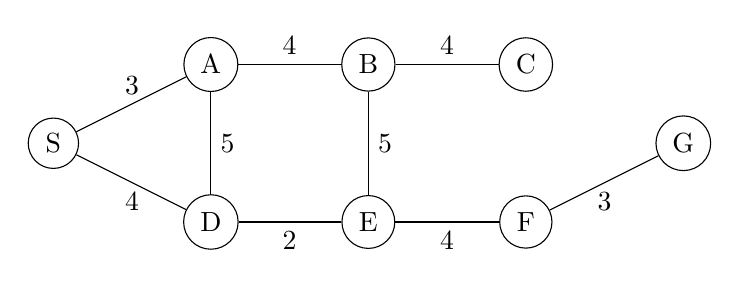
\begin{tikzpicture}
        \node [draw,circle](s)at(0,0){S};
        \node [draw,circle](a)at(2,1){A};
        \node [draw,circle](d)at(2,-1){D};
        \node [draw,circle](b)at(4,1){B};
        \node [draw,circle](e)at(4,-1){E};
        \node [draw,circle](c)at(6,1){C};
        \node [draw,circle](f)at(6,-1){F};
        \node [draw,circle](g)at(8,0){G};

        \draw (s) -- (a); 
        \draw (a) -- (b);
        \draw (b) -- (c);
        \draw (a) -- (d);
        \draw (s) -- (d);
        \draw (d) -- (e);
        \draw (b) -- (e);
        \draw (e) -- (f);
        \draw (f) -- (g);        

        \draw (1,1/2) node[above]{$3$};
        \draw (1,-1/2) node[below]{$4$};
        \draw (2,0) node[right]{$5$};
        \draw (3,1) node[above]{$4$};
        \draw (3,-1) node[below]{$2$};
        \draw (4,0) node[right]{$5$};
        \draw (5,1) node[above]{$4$};
        \draw (5,-1) node[below]{$4$};
        \draw (7,-1/2) node[below]{$3$};
    \end{tikzpicture}
    \caption{Path cost $g(n)$}
    \label{usc_path_cost}
\end{figure}

\begin{figure}[htbp]
    \centering
    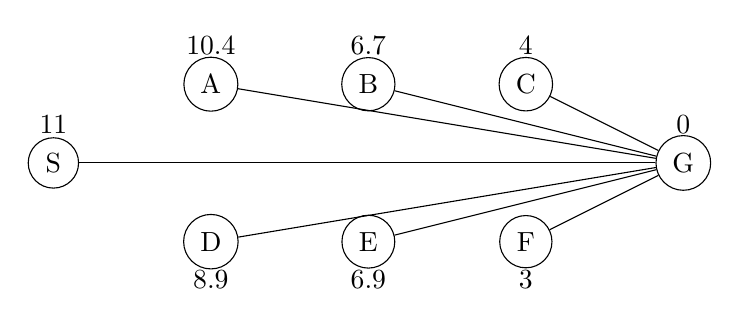
\begin{tikzpicture}
        \node [draw,circle](s)at(0,0){S};
        \node [draw,circle](a)at(2,1){A};
        \node [draw,circle](d)at(2,-1){D};
        \node [draw,circle](b)at(4,1){B};
        \node [draw,circle](e)at(4,-1){E};
        \node [draw,circle](c)at(6,1){C};
        \node [draw,circle](f)at(6,-1){F};
        \node [draw,circle](g)at(8,0){G};

        \draw (s) -- (g);
        \draw (a) -- (g);       
        \draw (d) -- (g);
        \draw (b) -- (g);
        \draw (e) -- (g);
        \draw (c) -- (g);
        \draw (f) -- (g);

        \draw (0,1/4) node[above]{$11$};
        \draw (2,5/4) node[above]{$10.4$};
        \draw (2,-5/4) node[below]{$8.9$};
        \draw (4,5/4) node[above]{$6.7$};
        \draw (4,-5/4) node[below]{$6.9$};
        \draw (6,5/4) node[above]{$4$};
        \draw (6,-5/4) node[below]{$3$};
        \draw (8,1/4) node[above]{$0$};
    \end{tikzpicture}
    \caption{Heuristic $h(n)$}
    \label{greedy_search_heuristic}
\end{figure}

\noindent
However, this is not enough for optimal. We need to do something on the heuristic cost. Otherwises, the actual bad goal cost < estimated good goal cost. \textbf{Admissible heuritics} is needed, they \textbf{underestimate the actual cost}. Saying that $h$ is admissible iff for all nodes $n \le h(n) \le h^{*}(n)$ where $h^{*}(n)$ is the actual cost to the closest goal. \\
How to come up with admissible heuristics? The cost of an optimal solution to a \textbf{relaxed problem} is admissible heuristics, an understimate, for the original problem. \\
Larger admissible heuristics, better estimation, closer to actual value, \textcolor{red}{but cannot larger than actual value (upper bound).} For example, $h2$ dominates $h1$ means for all nodes $n: h2(n) \ge h1(n)$. In this case, $h2$ is always better than $h1$, but for all nodes $h1(n) \le h2(n) \le h^{*}(n)$. For two heuristics $h1$ and $h2$, $h3(n) = max(h1(n),h2(n))$ always dominates both $h1$ and $h2$, because for all nodes n, $h3(n) \ge h1(n)$ and $h3(n) \ge h1(n)$.

\subsection{Summary}
\begin{enumerate}
    \item The best heuristics $f(n) = g(n) + h(n)$ is an \textbf{admissble heuristics} with the combination of Uniformed Cost Search and Greedy Search.
    \item Coming up with a good admissible heuristics is important (larger -> better -> closer to the $h^{*}(n)$ (actual value), but also should be (for all nodes n) smaller than $h^{*}(n)$)
\end{enumerate}

\pagebreak
\section{CSP}

\section{Pattern mining}

\section{Game tree}

\section{Planing}

\section{MDP}

\clearpage


\end{document}
